\subsection{Popularity of Resource}
\label{popularity of resource}
\paragraph{Motivation.}
It seems reasonable to assume that users have a tendency to click on links to articles that are describing trending and popular topics. This is the motivation for constructing the features described below.

Each of the features consists of a numerical measure estimating the degree of user interest for the resource article $\beta$ in the pair $(p, \beta)$.

\paragraph{Restrictions.}
For our model to be applicable to new articles, we should not, in general, use any information on article $p$ that is generated by user behavior. If we were to use such information we would not, in practice, be able to correctly apply our model to new articles before sufficient data had been logged. In other words, if we for example had, in our model, included information on the volume of social traffic for both articles in the pair, then we would not be ably to compute all feature values before query logs had generated sufficient data for both articles. 

Furthermore, we limit ourselves to using traffic data from external and well known sources and not include data from internal Wikipedia searches or when the referrer is missing, which could possibly be due to spoofed referral headers. We take these precautions to avoid potential unwanted bias.

% * <blandine.seznec@gmail.com> 2016-05-31T13:19:16.978Z:
%
% I don't understand what kind of information we're talking about and in what way it can cause a problem.
%
% ^ <philip@thruesen.dk> 2016-06-01T17:05:36.480Z:
%
% I've tried to elaborate
%
% ^ <jarekcechak@gmail.com> 2016-06-02T08:28:56.763Z.

\paragraph{Description.}
From the clickstream data it is possible to derive the number of article views on an article that are as a result of external traffic i.e. traffic coming from outside the Wikipedia domain. This gives us the possibility of extracting the number of searches from known search providers: Google, Bing and Yahoo! or the number of visits from social media sites such as Twitter and Facebook. This is traced using the HTTP header information: `
``referer''. Note that this information is completely separated from the information used for creating the ground truth -- for that, only internal click counts were used.

We consider traffic from search and social media individually. \cite{teevan2011twittersearch} states that users might have different intentions depending on from which media they choose to search or browse for content. For example,  users on social media tend to look for content that is currently trending and relevant in a temporal context, whereas typical search engine queries tend to be more about basic facts and general knowledge.

Discussions and illustrations in the following sections are for brevity and without loss of generality only focused on ``interest'' measures acquired from search engines -- Performing the same feature construction and processing on social media data gives comparable results, but given that the search engine data were more comprehensive and had fewer instances filtered by the 10-count rule of the clickstream dataset, it was selected for proof of concept.
% * <roelcastanomoreno@gmail.com> 2016-05-31T13:16:24.759Z:
%
% > without loss of generality
%
% Not sure what this means
%
% ^ <philip@thruesen.dk> 2016-06-01T15:15:02.043Z:
%
% a term you use when you prove something on a specific case but want the reader to know that it also applies to the general case.
%
% ^ <jarekcechak@gmail.com> 2016-06-02T08:30:43.195Z.
\paragraph{Feature Construction.}
Let the number of page views of an arbitrary article, $\sigma$, originated from searches from external search engines, be denoted as $search(\sigma)$ -- This is referred to as search interest (or simply interest).

Social networks are known for ``virally'' spreading topics that in terms of popularity or ``shares'' will follow a power law distribution \cite{jain2014scalable} -- this is a consequence of social networks forming scale-free graphs. Assuming interest in articles from both search- and social media sites have emerged from, and is driven by, social networks, we consider that our distribution of article views from these external sources are as such.

\begin{figure}[H]
\centering
    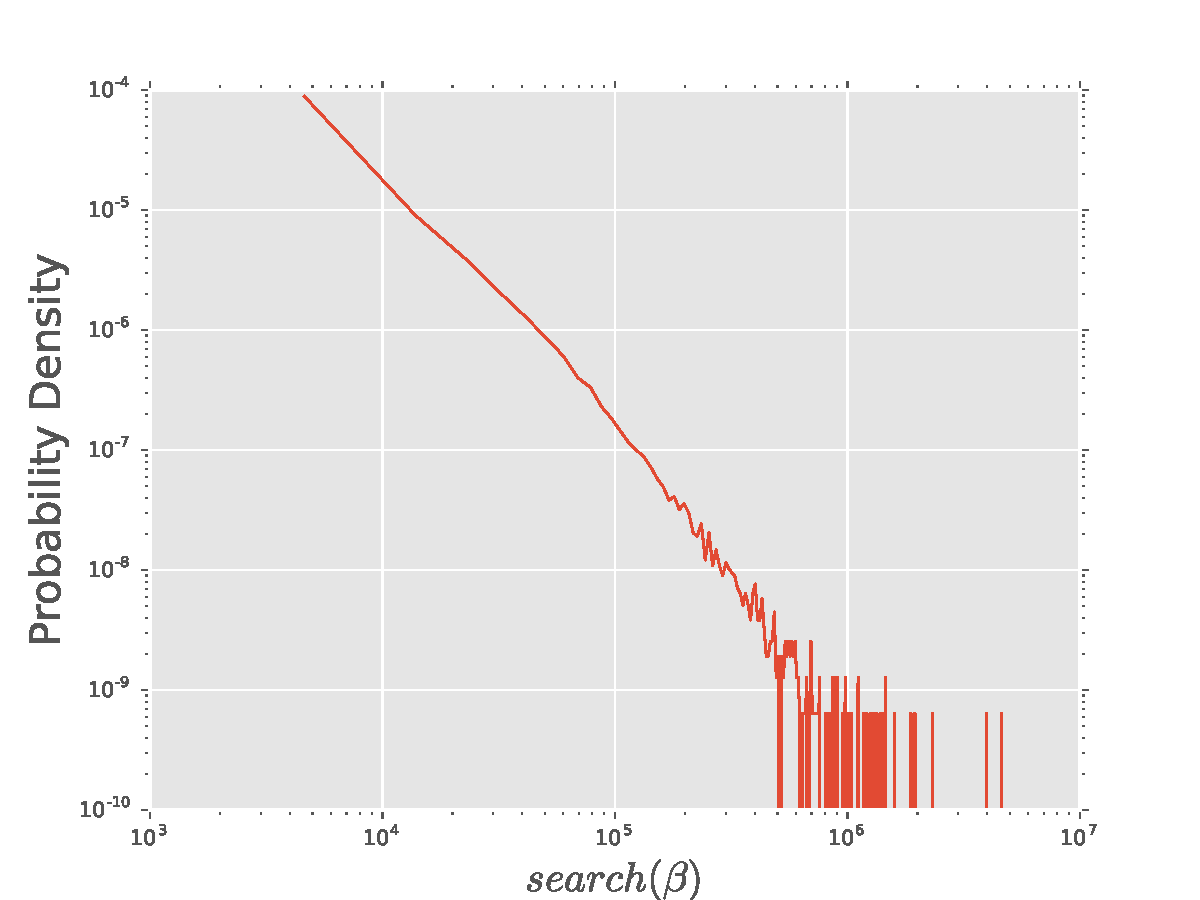
\includegraphics[width=0.47\textwidth]{images/loglog}
 \captionof{figure}{Log-log plot of search interest in articles. The articles used for plotting are the set of all $\beta$-articles. Note how the plot appear linear to support the theory of a power law distribution.}
 \label{fig:loglog}
\end{figure}

\medskip

The nature of the power law distribution results in the number of popular links (referred articles) being extremely small compared to the number of links in total. To illustrate that our above assumptions for distribution of interest holds, figure \ref{fig:loglog} shows how the probability density function of article search interest are linear in a log-log plotting which is characteristic for the power law distributions (aka. the power law signature).




Given the distribution of article interest we construct a feature $f_{search}$ for an article pair $(p_r, \beta_s)$. It is defined by the log of the measured interest, $search(\beta_s)$, after which we normalize by dividing with the maximal interest for articles in the set $B_r$ containing all articles referenced to from prominent article $p_r$. Eq. \ref{eq:fsearch} formalizes this where, naturally, we account for not taking log of zero.

\begin{multline}
f_{search}(p_r, \beta_s) = \\
\begin{cases}
      \displaystyle \frac{\log search(\beta_s)}{ \log \displaystyle \max_{\forall \beta \in B_r} search(\beta)}, & \text{if}\ search(\beta_s)>0 \\
      0, & \text{otherwise}
    \end{cases}
    \label{eq:fsearch}
\end{multline}
We perform the above calculation to counter-effect the nature of the power law so we consequently have a more linear feature as an outcome.
%\paragraph{Evaluation.}
%The final outcome of this processing results in the feature having a correlation coefficient of $r = 0,3879$ and a `coefficient of determination' of $r^2 = 0,15$. 

\subsection{Popularity Percentile Rank}
\label{popularity percentile rank}
In the previous section a feature $f_{search}$ was introduced. In this section we introduce a feature based on the same data but rather than processing ``raw'' interest values we focus more on internal ranking of subsets of articles. We denote this feature by $f'_{search}$.

\paragraph{Motivation.}
One could argue that this feature would be much similar to the previous but as these data have already proven to be useful we may reduce noise and improve class separation by adding features with somewhat correlated (and presumably semi-redundant) values \cite{guyon2003introduction}.

\paragraph{Description.}
We define $f'_{search}$ for an article pair $(p, \beta)$ as the probability that a randomly selected article $\mathcal{R}$ has a lower interest value than $\beta$, where $\mathcal{R} \neq \beta$ and $B$ is the set of all articles referenced from prominent article $p$ where $\{\mathcal{R}, \beta\} \subseteq B$. 
\begin{align}
f'_{search}(p, \beta) = pr(search(\mathcal{R}) < search(\beta))
\label{eq:search2}
\end{align}

We assume for the following that all articles have distinct values of interest. What is characteristic about this feature is that when $search(\beta_k)$ is the maximal value for any article in $B$ then the feature values is $1$ (eq. \ref{eq:fsearch2_m}). Furthermore when we are computing for the least interesting article or the article on the median we get respectively $0$ and $0.5$.
\begin{multline}
f'_{search}(p, \beta_k) = 
\begin{cases}
      0, & \text{if}\ \displaystyle \min_{\forall \beta \in B} search(\beta) = search(\beta_k) \\
      0.5, & \text{if}\ \displaystyle \med_{\forall \beta \in B} search(\beta) = search(\beta_k) \\
      1, & \text{if}\ \displaystyle \max_{\forall \beta \in B} search(\beta) = search(\beta_k)
    \end{cases}
    \label{eq:fsearch2_m}
\end{multline}

%\paragraph{Evaluation.}
%Correlating this feature with the rank of the ground truth the correlation coefficient yields $r = 0.138$ -- This is a small improvement over the other interest feature.
